\documentclass[11pt,letterpaper]{article}

% ---- fonts and page ---------------------------------------------------------------------------------------------
\usepackage[T1]{fontenc}
\usepackage[utf8]{inputenc}
\usepackage{newtxtext}
\usepackage{newtxmath}
\usepackage[letterpaper,top=0.60in,left=0.65in,right=0.65in,bottom=0.65in]{geometry}
\usepackage{microtype}
\usepackage{newunicodechar}
\newunicodechar{→}{\ensuremath{\rightarrow}}
\newunicodechar{×}{\ensuremath{\times}}
\newunicodechar{−}{\ensuremath{-}}
\newunicodechar{·}{\textperiodcentered}
\newunicodechar{…}{\ldots}

% ---- paragraphs and headings: justified, no indent, ~3 pt between paragraphs, compact headings --------------------
\setlength{\parindent}{0pt}
\setlength{\parskip}{3pt plus 1pt}
\usepackage{titlesec}
\titleformat{\section}{\normalfont\large\bfseries}{\thesection}{0.6em}{}
\titleformat{\subsection}{\normalfont\normalsize\bfseries}{\thesubsection}{0.6em}{}
\titleformat{\subsubsection}[runin]{\normalfont\normalsize\bfseries}{}{0pt}{}[.]
\titlespacing*{\section}{0pt}{8pt plus 2pt minus 1pt}{3pt plus 1pt}
\titlespacing*{\subsection}{0pt}{6pt plus 2pt minus 1pt}{2pt plus 1pt}
\titlespacing*{\subsubsection}{0pt}{4pt plus 1pt}{0.6em}
\widowpenalty=10000 \clubpenalty=10000 \displaywidowpenalty=10000
\setlength{\emergencystretch}{3em}

% ---- tables, figures, lists -------------------------------------------------------------------------------------
\usepackage{booktabs}
\usepackage{array}
\usepackage{calc}
\usepackage{tabularx}
\usepackage{multirow}
\usepackage{graphicx}
\usepackage{float}
\usepackage[font=small,labelfont=bf,skip=3pt]{caption}
\setlength{\textfloatsep}{8pt plus 2pt minus 2pt}
\setlength{\floatsep}{6pt plus 2pt minus 2pt}
\setlength{\intextsep}{6pt plus 2pt minus 2pt}
\usepackage{enumitem}
\setlist{nosep,leftmargin=1.2em}
\usepackage{xcolor}
\usepackage{pgfplots}
\pgfplotsset{compat=1.18}
\usetikzlibrary{patterns,arrows.meta,positioning,fit,calc}
\usepackage{fvextra}
\usepackage{needspace}
\usepackage{xurl}
\usepackage[hidelinks]{hyperref}
\newcolumntype{Y}{>{\raggedright\arraybackslash}X}
\providecommand{\tightlist}{\setlength{\itemsep}{0pt}\setlength{\parskip}{0pt}}
\newcommand{\repo}{\url{https://github.com/atlasmarkz/tacc-agentforge}}
\newcommand{\keybox}[1]{\par\noindent\fbox{\parbox{\dimexpr\linewidth-2\fboxsep-2\fboxrule}{#1}}\par}
\graphicspath{{../}{build/}}

\begin{document}

% ---- title ------------------------------------------------------------------------------------------------------
\begin{center}
{\LARGE\bfseries TACC AgentForge: A Budget-Verified Shopping Agent\\[2pt] on a Quantized 27B Model}\\[6pt]
{\large CSIT6000V Advanced AI Computing and Systems --- Course Project Report and Repository Submission}\\[4pt]
Hechuan Zhang \quad Berlin Chen \quad Jieming Chen\\[3pt]
\textbf{Repository:} \repo\\[1pt]
{\small Evaluated system: commit \texttt{cc6059d} (freeze digest \texttt{03b0cdea}); repository README: Appendix~\ref{app:readme}}
\end{center}

\section{Introduction}\label{sec:intro}

TACC AgentForge is a shopping and budget advisor. A user states what they need and how much they can spend; an agent
searches a source-linked product catalog, compares offers, checks the plan against the budget with exact decimal
arithmetic, and explains the recommendation with citations. The model is the course-provided Qwen3.8-27B AWQ INT4
checkpoint, served by vLLM on two GPUs on the TACC cluster. The project covers the whole stack: data collection and a
versioned knowledge base, the agent and its budget validator, model serving with hourly job handover, a browser
application, an evaluation with independent ground truth, serving optimizations, and a post-training pilot.

Table~\ref{tab:claims} lists the results this report makes. Every number is recomputed from committed raw data by one
command (Section~\ref{sec:artifact}); the repository README (Appendix~\ref{app:readme}) uses the same IDs C1--C7.

\begin{table}[H]
\centering\small
\caption{Main results. Section and table numbers refer to this report.}\label{tab:claims}
\begin{tabularx}{\linewidth}{@{}l Y l@{}}
\toprule
ID & Result & Where \\
\midrule
C1 & On 32 held-out cases $\times$ 3 repeats the full agent (B3v) succeeds in \textbf{42/96} attempts; single-call baselines reach 54--57/96. & \S\ref{sec:agent-results}, Table~\ref{tab:heldout} \\
C2 & The budget validator helps: B3$\rightarrow$B3v paired difference \textbf{+0.10} (95\% CI +0.02 to +0.20); no configuration delivers an over-budget plan. & \S\ref{sec:agent-results}, Table~\ref{tab:heldout} \\
C3 & The agent wins where searching is needed (plan cases 33/60 vs.\ at most 21/60) but \textbf{48/96} runs stop at the 8-call limit. & \S\ref{sec:agent-results}, Fig.~\ref{fig:outcome}, Table~\ref{tab:failures} \\
C4 & CUDA graphs give \textbf{+202\%} output throughput over eager mode; prefix caching cuts TTFT by 71\% on shared prefixes. & \S\ref{sec:serving}, Table~\ref{tab:serving}, Fig.~\ref{fig:serving} \\
C5 & A one-line vLLM fix makes MTP speculative decoding work with CUDA graphs: \textbf{+42\%} single-request throughput. & \S\ref{sec:mtp}, Table~\ref{tab:mtp} \\
C6 & SFT pilot: a LoRA adapter picks the correct category in \textbf{8/8} first steps vs.\ 2/8 (pipeline check only). & \S\ref{sec:sft}, Table~\ref{tab:sft} \\
C7 & Post-freeze fix of the call limit: no-plan case ends in 3 calls instead of 8, in all 9 targeted replays. & \S\ref{sec:fix}, Table~\ref{tab:replay} \\
\bottomrule
\end{tabularx}
\end{table}

\keybox{\textbf{Main finding.} Exact budget validation works --- no over-budget plan was ever delivered --- but a
multi-step agent with an 8-call budget loses to a single well-prompted call overall, because it does not stop
searching when no feasible offer exists. A targeted fix after the freeze removes this failure in replays; the
held-out split has not been rerun with it.}

\section{System}\label{sec:system}

\begin{figure}[t]
\centering
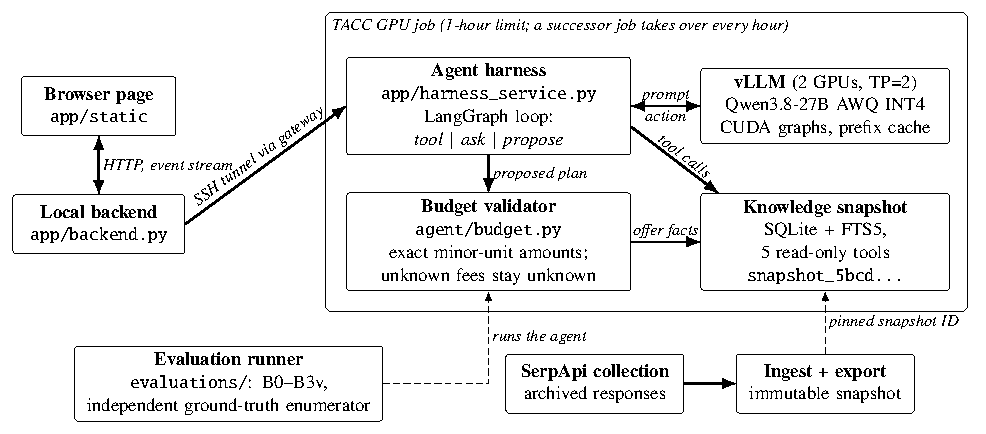
\includegraphics[width=0.94\linewidth]{report/figures/architecture-standalone.pdf}
\caption{The evaluated deployment. The browser reaches the agent on the cluster through a local backend and an SSH tunnel; one TACC GPU job runs the agent harness, the budget validator, vLLM and the pinned knowledge snapshot. Dashed: offline data pipeline and evaluation.}\label{fig:arch}
\end{figure}

\textbf{Knowledge base.} SerpApi Google Shopping and Google Product responses are archived verbatim with their
request parameters and hashes, normalized into SQLite with FTS5 full-text search, and exported as an immutable
snapshot whose ID is a hash of its content. The evaluated snapshot \texttt{snapshot\_5bcd00723fb0b7589cbe50c8} holds
four categories (earbuds, chargers, keyboards, backpacks), 315 discovered product groups, 80 with full details, 251
offers, 380 reviews, 2{,}507 attributes and 3{,}525 source-linked evidence records. Attributes are stored only when the
source states them; unknown, range and conflicting values stay unknown instead of being guessed. The agent reaches
the snapshot through five tools: \texttt{describe\_filters}, \texttt{search\_products}, \texttt{retrieve\_evidence},
\texttt{get\_offer\_facts} and \texttt{resolve\_evidence}; results are size-bounded and paginated.

\textbf{Agent and budget validator.} The agent is a LangGraph loop. At each step the model must emit one JSON action
--- call a tool, ask the user, or propose a plan --- and decoding is constrained to the action schema. Runs are bounded
by 8 model calls, 8 tool calls, two repairs of invalid actions, a 120-second budget and a 36{,}000-character context.
A proposed plan is only delivered after the \emph{budget validator} approves it: it recomputes every line in minor
currency units from the snapshot's offer facts, takes the smaller of the purchase cap and the periodic budget after
spending and reserves, compares before tax by default and says so, and treats unknown shipping or tax as unknown
rather than zero. If a required budget field is missing the run pauses with a question; checkpoints let the user's
answer resume it. After approval the model streams a short explanation; numbers in it must come from the verified plan
or the cited evidence, otherwise a template answer replaces it.

\textbf{Serving on TACC.} vLLM runs with tensor parallelism 2, a 16{,}384-token context, prefix caching and CUDA
graphs. Jobs are limited to one hour, so a running service submits its successor 15 minutes before its limit and
withdraws its address only after the successor is ready; in a 30-minute soak with one request every 30 seconds, none
of the 60 requests failed because of the handover. Startup takes 5 to 8.5 minutes. The job scripts handle two cluster quirks: GPUs
held by processes outside Slurm, and nodes whose allocated GPU IDs do not match the IDs visible inside the job.

\textbf{Application.} A browser page talks to a local backend, which reaches the agent service on the cluster through
an SSH tunnel and relays its event stream, so the user sees each step (search, comparison, budget check,
explanation). A request with a budget took 18\,s end to end, with the first event after 0.4\,s; Fig.~\ref{fig:ui}
shows the result page.

\begin{figure}[t]
\centering
\includegraphics[width=0.52\linewidth]{build/browser-demo.png}
\caption{Result page with the real model on TACC: one verified offer at \$22.99 before tax, \$77.01 left of a \$100 budget, the explanation with evidence references, and the source.}\label{fig:ui}
\end{figure}

\section{Evaluation Method}\label{sec:method}

\textbf{Cases.} 42 cases in English and Chinese over the four categories: 10 development and 32 held-out (8 per
category). By expected outcome the held-out split has 20 cases that need a plan, 8 with no feasible plan and 4 that
must ask for the budget. Ground truth is computed, not written by hand: an independent enumerator reads the snapshot's
SQLite file directly and does not use the agent's tools or validator.

\textbf{Configurations.} All use temperature 0, thinking off and JSON output; each case runs every configuration in a
rotated order, three times.

\begin{table}[H]
\centering\small
\caption{Configurations.}\label{tab:configs}
\begin{tabularx}{\linewidth}{@{}l Y@{}}
\toprule
Name & Description \\
\midrule
B0 & One model call with the 10 cheapest in-budget candidates of the category \\
B1 / B2 & B0 plus the top 5 evidence records from keyword / filtered retrieval \\
B3 & Multi-step agent with the real tools; the validator is replaced by a recorder (ablation) \\
B3v & \textbf{Full system}: B3 plus the real budget validator; only approved plans count as delivered \\
\bottomrule
\end{tabularx}
\end{table}

\textbf{Metrics.} Task success rate (TSR): the outcome matches the ground truth (a feasible plan, the correct ``no
feasible plan'', or asking for the budget). Budget violation rate (BVR): delivered plans over budget. We also count
constraint violations, unverifiable claims (a required attribute of the chosen offer is unknown) and made-up IDs.
Confidence intervals are per-case bootstrap 95\% intervals; paired differences compare configurations case by case.
The evaluated system is frozen: the runner refuses the held-out split unless every evaluated file matches the freeze
manifest.

\section{Results}\label{sec:results}

\subsection{Agent evaluation (C1--C3)}\label{sec:agent-results}

\begin{table}[H]
\centering\small
\caption{Held-out results: 32 cases $\times$ 3 repeats = 96 attempts per configuration. Expected-outcome columns give successes per outcome type. Paired per-case differences (95\% CI): B0$\rightarrow$B1 +0.03 (0.00 to 0.09); B1$\rightarrow$B2 0.00; B2$\rightarrow$B3 $-$0.26 ($-$0.47 to $-$0.05); \textbf{B3$\rightarrow$B3v +0.10 (+0.02 to +0.20)}.}\label{tab:heldout}
\setlength{\tabcolsep}{5pt}
\begin{tabular}{@{}l r c r r r r r@{}}
\toprule
& & Per-case mean & \multicolumn{3}{c}{By expected outcome} & & \\
\cmidrule(lr){4-6}
Config & TSR & (95\% CI) & Plan & No plan & Ask & BVR & Unverif. \\
\midrule
B0 & 54/96 & 0.56 (0.38--0.72) & 18/60 & 24/24 & 12/12 & 0/25 & 7/25 \\
B1 & 57/96 & 0.59 (0.44--0.75) & 21/60 & 24/24 & 12/12 & 0/27 & 6/27 \\
B2 & 57/96 & 0.59 (0.44--0.75) & 21/60 & 24/24 & 12/12 & 0/26 & 5/26 \\
B3 & 32/96 & 0.33 (0.19--0.50) & 29/60 & 0/24 & 3/12 & 0/42 & 7/42 \\
\textbf{B3v} & \textbf{42/96} & \textbf{0.44 (0.28--0.60)} & \textbf{33/60} & 0/24 & 9/12 & 0/36 & 3/36 \\
\bottomrule
\end{tabular}
\end{table}

\textbf{C1.} The full agent succeeds in 42 of 96 attempts; adding retrieval to a single call gives 57/96. No
configuration violated a hard constraint or invented an ID. \textbf{C2.} Adding the validator to the agent raises TSR
by 0.10 per case, and its interval excludes zero. Most of the gain is on cases that must ask for the budget (3/12
$\rightarrow$ 9/12): without the validator the agent proposed plans without knowing the budget six times. No
configuration delivered an over-budget plan (BVR 0 everywhere).

\begin{figure}[H]
\centering
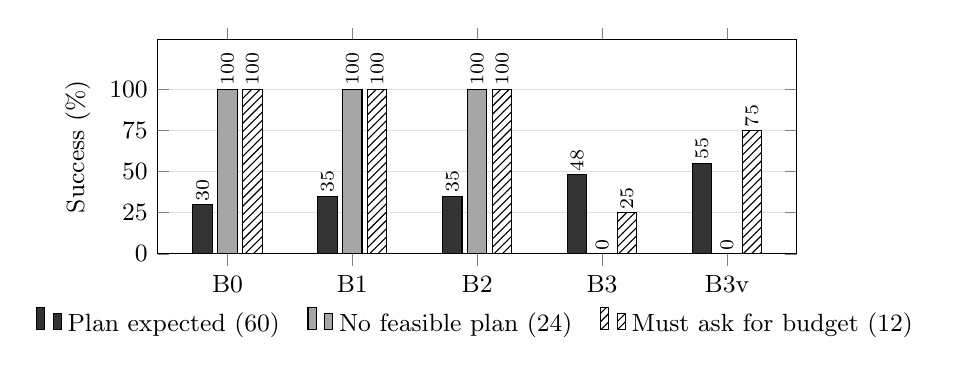
\begin{tikzpicture}
\begin{axis}[
  ybar, width=0.80\linewidth, height=4.3cm, bar width=7pt, ymin=0, ymax=130, ytick={0,25,50,75,100},
  ylabel={Success (\%)}, ylabel style={font=\small}, tick label style={font=\small},
  symbolic x coords={B0,B1,B2,B3,B3v}, xtick=data, enlarge x limits=0.14,
  legend style={font=\small, at={(0.5,-0.22)}, anchor=north, legend columns=3, draw=none, /tikz/every even column/.append style={column sep=8pt}},
  nodes near coords, every node near coord/.append style={font=\scriptsize, rotate=90, anchor=west, inner sep=1pt},
  ymajorgrids, grid style={gray!25}]
\addplot[fill=black!80, draw=black] coordinates {(B0,30) (B1,35) (B2,35) (B3,48) (B3v,55)};
\addplot[fill=black!35, draw=black] coordinates {(B0,100) (B1,100) (B2,100) (B3,0) (B3v,0)};
\addplot[fill=white, draw=black, postaction={pattern=north east lines}] coordinates {(B0,100) (B1,100) (B2,100) (B3,25) (B3v,75)};
\legend{Plan expected (60), No feasible plan (24), Must ask for budget (12)}
\end{axis}
\end{tikzpicture}
\caption{Held-out success by expected outcome (percent of attempts). The agent wins where a plan must be found by searching, and fails every case without a feasible plan.}\label{fig:outcome}
\end{figure}

\textbf{C3.} The agent is better where a plan has to be found (33/60 vs.\ at most 21/60): single calls only see the 10
cheapest candidates and asked unnecessary questions 33--35 times. It loses overall because half of its runs end at
the model-call limit, including 22 of 24 runs on cases without a feasible plan (Table~\ref{tab:failures}).

\begin{table}[H]
\centering\small
\caption{Failure reasons on the held-out split (attempts out of 96 per configuration).}\label{tab:failures}
\begin{tabular}{@{}l r r r r r@{}}
\toprule
Reason & B0 & B1 & B2 & B3 & B3v \\
\midrule
Stopped at the 8-call model limit & -- & -- & -- & 48 & \textbf{48} \\
Unnecessary clarification question & 35 & 33 & 34 & -- & -- \\
Unverifiable claim (required attribute unknown) & 7 & 6 & 5 & 4 & 1 \\
Plan proposed although the budget was missing & -- & -- & -- & 6 & -- \\
Asked, but not for the budget & -- & -- & -- & 3 & 3 \\
Plan proposed although none is feasible & -- & -- & -- & 3 & 2 \\
\bottomrule
\end{tabular}
\end{table}

Traces show the mechanism. Searches include items whose price or attributes are unknown, so a query with no feasible
offer still returns pages of candidates and a next-page cursor; the model keeps paging instead of concluding that
nothing fits, and each page costs a model call. Every observation is about 8.5K characters, so the 36K-character
context keeps only about three pages. The agent also has no notion of its remaining budget. Cost follows: B3v uses 6.5
model calls and about 37K prompt tokens per request (single calls: 1 call, about 7K tokens), with a median latency of
19\,s and p95 of 37\,s versus 3--4\,s for single calls.

\subsection{Post-freeze fix of the call limit (C7)}\label{sec:fix}

After the freeze (PR \#29) the agent reserves its last two calls for finishing, finishes after two consecutive steps
without progress, runs a repeated read-only query only once, and may end early with ``no feasible plan in this
catalog''; the hard limit stays at 8 calls. Replays with the real model on three requests, three times each:

\begin{table}[H]
\centering\small
\caption{Targeted replays after the fix (model calls and end state; identical in all three repeats). Rerun on 2026-11-19 from a fresh clone with the same result.}\label{tab:replay}
\begin{tabular}{@{}l l l@{}}
\toprule
Request & Frozen system & After the fix \\
\midrule
dev-07 (keyboard under 10 USD; none) & 8 calls, call limit & \textbf{3 calls, \texttt{no\_feasible\_plan}} \\
dev-04 (plan exists, 50 USD) & 5 calls, completed & 5 calls, completed with a verified plan \\
Issue-21 charger request (60 USD) & 12/12 runs at the call limit & 1 call, asks for the laptop's power need \\
\bottomrule
\end{tabular}
\end{table}

These are 9 targeted runs, not a held-out rerun, so the report claims no new overall TSR.

\subsection{Serving optimizations (C4)}\label{sec:serving}

Each variant changes one vLLM flag from an eager-mode baseline (one node, two GPUs; 8 prompts $\times$ 2 repeats per
stage, 128 output tokens; concurrency 8 shown).

\begin{table}[H]
\centering\small
\caption{Serving variants, distinct prompts, concurrency 8 (eager baseline). Changes are relative to the baseline of the same job.}\label{tab:serving}
\begin{tabular}{@{}l r r r l@{}}
\toprule
Variant & Output tok/s & TTFT p50 (ms) & TPOT p50 (ms) & Note \\
\midrule
Baseline (eager) & 67.4 & 1474 & 103.3 & \\
\textbf{CUDA graphs} & \textbf{203.9} (+202\%) & 1727 & \textbf{25.8} ($-$75\%) & largest gain \\
Prefix caching & 71.9 (+7\%) & 1476 & 96.1 & shared prefix: TTFT 2274$\rightarrow$654\,ms \\
No chunked prefill & 72.3 (+7\%) & 2135 & 92.7 & TTFT +45\% \\
Triton attention & 66.1 & 1941 & 104.1 & TTFT +32\% \\
FlashInfer attention & \multicolumn{3}{c}{failed (engine died after start)} & \\
FP8 KV cache & \multicolumn{3}{c}{failed (HTTP 500 on every request)} & \\
\bottomrule
\end{tabular}
\end{table}

\begin{figure}[H]
\centering
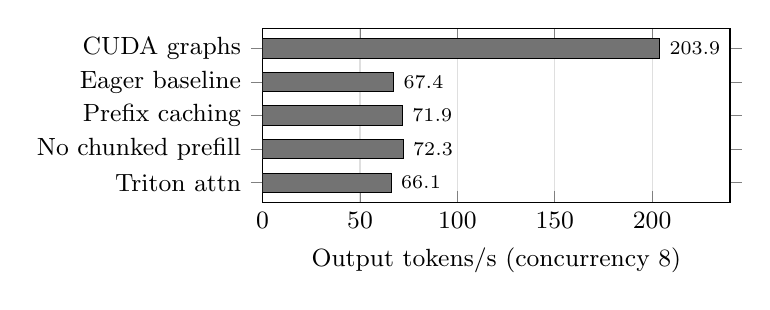
\begin{tikzpicture}
\begin{axis}[
  xbar, width=0.62\linewidth, height=3.8cm, bar width=7pt, xmin=0, xmax=240,
  xlabel={Output tokens/s (concurrency 8)}, xlabel style={font=\small}, tick label style={font=\small},
  symbolic y coords={Triton attn,No chunked prefill,Prefix caching,Eager baseline,CUDA graphs}, ytick=data,
  nodes near coords, nodes near coords style={font=\scriptsize}, enlarge y limits=0.15,
  xmajorgrids, grid style={gray!25}]
\addplot[fill=black!55, draw=black] coordinates {(66.1,Triton attn) (72.3,No chunked prefill) (71.9,Prefix caching) (67.4,Eager baseline) (203.9,CUDA graphs)};
\end{axis}
\end{tikzpicture}
\caption{Output throughput of the serving variants (distinct prompts). CUDA graphs dominate; the other flags change throughput by at most 7\%.}\label{fig:serving}
\end{figure}

With CUDA graphs as the new baseline, the same flags change throughput by less than 3\% (203.5 tok/s baseline). The
deployed service therefore uses CUDA graphs and prefix caching (the agent's prompts share long prefixes).

\subsection{Speculative decoding with MTP (C5)}\label{sec:mtp}

With the course's private vLLM build, multi-token prediction (MTP) speculative decoding crashed during CUDA-graph
capture: the warm-up run built ordinary attention metadata, so a speculative-decoding Triton kernel was first compiled
inside stream capture, which CUDA forbids. A one-line change makes the warm-up build the same metadata as the
capture run.

\begin{table}[H]
\centering\small
\caption{Output tok/s with CUDA graphs and the fix (one measurement per cell; change vs.\ the graphs baseline).}\label{tab:mtp}
\begin{tabular}{@{}l r r r@{}}
\toprule
Workload & Baseline & MTP $k{=}1$ & MTP $k{=}3$ \\
\midrule
Distinct prompts, 1 request & 57.7 & 73.5 (+27\%) & \textbf{81.8 (+42\%)} \\
Shared prefix, 1 request & 37.6 & 44.2 (+18\%) & 47.9 (+27\%) \\
Distinct prompts, 4 requests & 139.5 & 129.0 ($-$8\%) & 136.8 ($-$2\%) \\
Shared prefix, 4 requests & 63.9 & 67.0 (+5\%) & 69.8 (+9\%) \\
\bottomrule
\end{tabular}
\end{table}

MTP reduces the latency of a lone request (mean acceptance length about 2.9 at $k{=}3$) but brings little throughput
under concurrency, where inter-token latency roughly doubles.

\subsection{Supervised fine-tuning pilot (C6)}\label{sec:sft}

To test the post-training pipeline, a LoRA adapter (rank 8, 54M trainable parameters) was trained on the INT4
checkpoint from successful development traces, with the category hint removed from the inputs, and served by vLLM next
to the base model. Of 69 examples, 31 fit the 4{,}096-token limit (26 train, 5 validation); training took 78 steps
(about 14 minutes), and validation loss rose after the first epoch.

\begin{table}[H]
\centering\small
\caption{First action on development prompts (temperature 0).}\label{tab:sft}
\begin{tabular}{@{}l c c@{}}
\toprule
Check & Base & LoRA adapter \\
\midrule
Correct catalog category on the first step (8 prompts with a budget) & 2/8 & \textbf{8/8} \\
\quad of which not seen in training (4 prompts) & 1/4 & 4/4 \\
Asks for a missing budget on the first step (2 prompts) & 1/2 & 0/2 \\
\bottomrule
\end{tabular}
\end{table}

This shows that the pipeline works end to end (traces $\rightarrow$ training on INT4 $\rightarrow$ vLLM serving) and that
the category-name defect can be trained away. It is \textbf{not a quality result}: 10 prompts from the development
split, first action only, and the adapter memorized a tiny dataset.

\section{Limitations}\label{sec:limits}

\begin{itemize}
\item \textbf{Call limit.} The frozen system's main failure (C3). The fix (C7) is supported by 9 replays only.
\item \textbf{The validator checks money, not requirements.} It approved three plans whose required attribute was unknown.
\item \textbf{Correctness is relative to the frozen snapshot.} All 251 offers have unknown tax, so budgets are compared before tax; known data errors carry into the ground truth.
\item \textbf{Small samples.} 32 held-out cases; single-call repeats are identical at temperature 0, so they give 32 independent results. Serving and MTP cells are single measurements.
\item \textbf{Not done.} New quantization (all results use the course's AWQ INT4 model), the fifth unseen category, human ratings of explanations, and retrieval Recall/MRR (the relevance pool is unlabeled).
\item \textbf{Variation.} vLLM batching is not bit-deterministic, so a TACC rerun of multi-step attempts can differ; latency depends on the node.
\end{itemize}

\section{Artifact and Reproduction}\label{sec:artifact}

The repository is public at \repo. Its README (Appendix~\ref{app:readme}) follows the NSDI artifact structure.
\begin{itemize}
\item \textbf{Getting started, about 10 minutes, no GPU.} After installing the locked dependencies, one command
(\texttt{scripts/check\_artifact.py}) runs seven stages --- environment, catalog snapshot, 686 tests, harness self-test,
an end-to-end request through backend, agent, knowledge base and validator, recomputation of C1--C7, and the v1
benchmark data --- and prints \texttt{SUCCESS} per stage and \texttt{ALL 7 STAGES SUCCEEDED}. Verified from fresh
clones.
\item \textbf{Main results.} \texttt{scripts/reproduce\_results.py} rescores all 660 recorded agent attempts against the
frozen snapshot, regenerates the serving reports, and recounts C5--C7 from raw outputs; it prints \texttt{ALL MATCH}.
\item \textbf{Reruns on TACC (optional).} On 2026-11-19 we followed the README on the cluster from a fresh clone. The
quick agent rerun (frozen commit, development split) gave B0 7/10 and B3v 6/10 with three call-limit stops and BVR 0,
consistent with the frozen development results (B0 21/30, B3v 14/30); the C7 replays reproduced exactly. The check
also found that serving-experiment jobs failed on nodes with mismatched GPU IDs; the job scripts now renumber them.
\end{itemize}

\section{Group Contributions}\label{sec:contrib}

\begin{table}[H]
\centering\small
\begin{tabularx}{\linewidth}{@{}l Y@{}}
\toprule
Member & Contributions \\
\midrule
Hechuan Zhang & Model serving on TACC with automatic recovery, hourly handover and runbook; budget validator; evaluation cases, independent enumerator, scorer and frozen baseline; browser, backend and cluster bridge; serving and speculative-decoding experiments including the vLLM fix; SFT pilot; README, reproduction and artifact check; public cloud deployment (separate branch). \\
Berlin Chen & Agent runtime (LangGraph loop, tools, policies, checkpoints); convergence and explanation fixes; the post-freeze fix of the call limit (C7). \\
Jieming Chen & Knowledge base: SerpApi collection, SQLite/FTS5 snapshots, retrieval tools and offline bootstrap; tool error recovery and schema discovery; persistent session memory and bounded context selection; the additional v1 benchmark and ShoppingBench track. \\
\bottomrule
\end{tabularx}
\end{table}

\appendix
\setcounter{secnumdepth}{2}
\titleformat{\subsubsection}{\normalfont\normalsize\bfseries}{}{0pt}{}
\titlespacing*{\subsubsection}{0pt}{5pt plus 2pt}{2pt plus 1pt}
\titleformat{\paragraph}[runin]{\normalfont\normalsize\bfseries}{}{0pt}{}[.]
\section{Repository README}\label{app:readme}
{\small Full contents of \texttt{README.md} at the submitted commit, converted to this format. The animated demo is
shown as a single frame.}
\input{build/readme.tex}

\end{document}
